% !TeX spellcheck = en_US
\section{Problem 1}

%Τα contour lines της συνάρτησης $f(x,y)$ που δίνεται στην εκφώνηση παράγεται με τον ακόλουθο κώδικα MATLAB και πορουσιάζεται στην εικόνα~\ref{fig:prob_1_contour_lines}.
Contour lines of $f(x,y)$ given are produced with the following MATLAB code and are presented in figure~\ref{fig:prob_1_contour_lines}.

\begin{lstlisting}[]
function [Z] = plot_contour(start_num, end_num)
	
	x = linspace(start_num, end_num, 100);
	y = x;
	[X, Y] = meshgrid(x, y);
	Z = X.^2 + 4*X.*Y + Y.^2;
	contour(X, Y, Z, 40);
	xlabel('X');
	ylabel('Y');
end
\end{lstlisting}
\begin{figure}[h]
	\centering
	\begin{subfigure}{0.4\textwidth}
		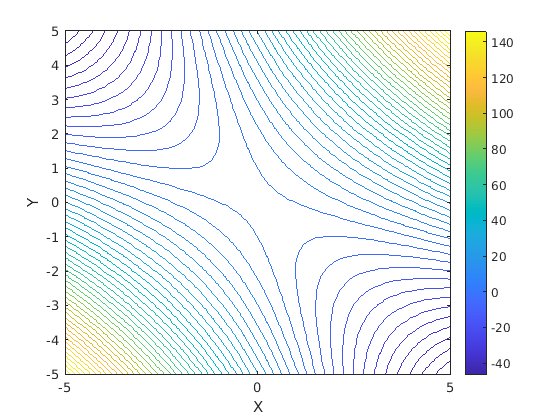
\includegraphics[width=\textwidth]{../Problem 1/contour_lines_2d.png}
		\caption{2D Plot}
		\label{fig:prob_1_contour_lines_2d}
	\end{subfigure}
	\begin{subfigure}{0.4\textwidth}
		\includesvg[width=\textwidth]{../Problem 1/contour_lines_3d.svg}
		\caption{3D Plot}
		\label{fig:prob_1_contour_lines_3d}
	\end{subfigure}
	\caption{Contour lines of $f(x,y)$ }
	\label{fig:prob_1_contour_lines}
\end{figure}

A general formula of a quadratic equation is $f(x,y) = ax^2 + 2bxy + cy^2$. Writing our formula in the previous form, we find that $a=1, \MathSpace b=2, \MathSpace c=1$.
Calculation of discriminant can help us calculate the location of function's local minimum/maximum.

\begin{equation}
\begin{gathered}
D =
\left[
\begin{array}{cc}
	f_{xx} & f_{xy} \\
	f_{yx} & f_{yy} \\
\end{array}
\right]
= f_{xx} f_{yy} - f^2_{xy} = 2 \times 2 - 4^2 = -12 < 0, \quad \text{όπου} \\
f_{xx} = \frac{\partial^2 f}{\partial x^2} = 2, \quad
f_{yy} = \frac{\partial^2 f}{\partial y^2} = 2, \quad
f_{xy} = \frac{\partial}{\partial y} \left( \frac{\partial f}{\partial x} \right) = 4
D = 2 \times 2 - 4^2 = -12 < 0.
\end{gathered}
\end{equation}

So, we only have to find the point where $\frac{\partial f}{\partial x}$ and $\frac{\partial f}{\partial y}$ are equal to $0$. Thus, this point will be a saddle point where gradients in each orthogonal direction are $0$, but this point is not either a local minimum or maximum.
Specifically:
\begin{equation}
\left\{
\begin{array}{c}
	\frac{\partial f}{\partial x} = 2x + 4y = 0 \\ 
	\frac{\partial f}{\partial y} = 4x + 2y = 0 \\
\end{array}
\right.
\Rightarrow
\left\{
\begin{array}{c}
	x = 0\\y=0\\
\end{array}
\right.
\end{equation}
Thus, the point $(x,y) = (0,0)$ is the saddle point mentioned before for the function given and this can be justified using the plotted contour lines.